\section{Ein-Teilchen-Greensfunktionen}\label{greensfkt}

In der Zeitdomäne ist die kausale Ein-Teilchen-Greensfunktion für Fermionen nach Gleichung \ref{1pgf} definiert.

\begin{equation}\label{1pgf}
G_{pq}(t,t') = -i \bra{\Psi_0^N}c_p(t)c_q^\dagger(t')\ket{\Psi_0^N}\Theta(t-t') +i \bra{\Psi_0^N}c_q^\dagger(t')c_p(t)\ket{\Psi_0^N}\Theta(t'-t)
\end{equation}

Bei $\Theta(t-t')$ (Gleichung \ref{stufe}) handelt es sich um die Stufenfunktion, die durch den Zeitordnungsoperator in der allgemeinen kausalen Greensfunktion entsteht.

\begin{equation}\label{stufe}
\Theta(t-t') = \begin{cases}
1 & \text{für } t>t'\\
0 & \text{für } t<t'
\end{cases}
\end{equation}

Abhängig von den Zeiten $t$ und $t'$ ist höchstens einer der Summanden aus Gleichung \ref{1pgf} von null verschieden. Für den Fall, dass $t'>t$ trägt nur der zweite Summand zur Greensfunktion bei. Er beschreibt die Wahrscheinlichkeitsamplitude, dass sich ein zur Zeit $t$ im Orbital $\ket{\phi_p}$ erzeugter Lochzustand zur späteren Zeit $t'$ im Orbital $\ket{\phi_q}$ befindet. Analog beschreibt die Greensfunktion für $t>t'$ die Propagation eines Teilchens. Aufgrund dieser Eigenschaft wird die Greensfunktion häufig auch \emph{Propagator} genannt.\cite{nolting7}

Aus dieser Betrachtungsweise ist auch ersichtlich, dass sich die Greensfunktion als Summe eines $N+1$- und eines $N-1$-Teils formulieren lässt:

\begin{equation}
G_{pq}(\omega) = G_{pq}^+(\omega) + G_{pq}^-(\omega)
\end{equation}

Die Greensfunktion \ref{1pgf} ist im Heisenbergbild gegeben, in dem die Operatoren zeitabhängig und die Zustände zeitunabhängig sind. Die Erzeugungs- und Vernichtungsoperatoren gehen damit über in $c_p(t) = \mathrm{e}^{-i\hamil t} c_p \mathrm{e}^{i\hamil t}$. Das Einfügen dieser zeitabhängigen Operatoren in die Greensfunktion des $N-1$-Teilchen-Systems und deren Wirken auf die Grundzustandswellenfunktion führt zu Gleichung \ref{g-hsb}.

\begin{equation}\label{g-hsb}
G_{pq}^-(t',t) = i\Theta(t'-t) \mathrm{e}^{iE_0^N(t'-t)}\bra{\Psi_0^N}c_q^\dagger\mathrm{e}^{-i\hamil(t'-t)}c_p\ket{\Psi_0^N}
\end{equation}

Mit einem zeitunabhängigen Hamiltonoperator $\hamil$ ist die Greensfunktion damit nur von der Zeitdifferenz $t'-t$ abhängig, $G_{pq}(t',t)$ geht also über in $G_{pq}(t'-t)$. Analog wird mit dem $N+1$-Teilchenteil verfahren.

Nach Einschieben einer vollständigen $N+1$-Teilchenbasis in $G_{pq}^+$ bzw. $N-1$-Teilchenbasis in $G_{pq}^-$ wird die Greensfunktion mittels einer Fouriertransformation von der Zeit- in die Energiedomäne überführt. Um die Konvergenz der Transformation zu gewährleisten wird der Faktor $\mathrm{e}^{-\eta(t'-t)}$ bzw. $\mathrm{e}^{-\eta(t-t')}$ eingeführt, bei dem $\eta$ eine infinitesimal kleine, positive Größe ist. Dieses führt zur Spektraldarstellung der Greensfunktion (Gleichung \ref{spektraldst}).

\begin{equation}\label{spektraldst}
G_{pq}(\omega) = \sum\limits_{n\in\{N+1\}}\frac{x_p^{(n)}x_q^{(n)*}}{\omega-e_n +i\eta} + \sum\limits_{n\in\{N-1\}}\frac{x_p^{(n)}x_q^{(n)*}}{\omega-e_n -i\eta}
\end{equation}

In dieser Darstellung wird der Zusammenhang mit den Ionisierungsspektren offensichtlich.  Die $e_n$ sind die Energiedifferenzen zwischen Anfangs- und Endzustand und korrespondieren somit mit den Ionisierungsenergien bzw. mit den Elektronenaffinitäten. Sie sind durch Auffinden der Polstellen der Greensfunktion ermittelbar. Die Polstärken $\left|x_p^{(n)}\right|^2$, die das Betragsquadrat der Übergangsamplituden $x_p^{(n)}=\bra{\Psi_n^{N-1}}c_p\ket{\Psi_0}$ sind, korrespondieren im zweiten Summanden mit der Wahrscheinlichkeit der entsprechenden Ionisierung.


Es sei noch erwähnt, dass Gleichung
\begin{equation}\label{fourier}
\begin{split}
G_{pq}(\omega) = \bra{\Psi_0^N}c_p(\omega+E_0^N-\hamil+i\eta)^{-1}c_q^\dagger\ket{\Psi_0^N} \\+ \bra{\Psi_0^N}c_q^\dagger(\omega-E_0^N+\hamil-i\eta)^{-1}c_p\ket{\Psi_0^N}
\end{split}
\end{equation}
in der Literatur häufig für die Greensfunktion angegeben wird. Bei ihr handelt es sich um die darstellungsfreie Form der Spektraldarstellung (\ref{spektraldst}).


\section{Zweiteilchen-Greensfunktion}
Analog zur Einteilchen-Greensfunktion existiert auch eine Zweiteilchen-Greensfunktion $\mathbf{\Pi}(\omega)$, mit deren Hilfe sich die Energiedifferenz zwischen einem $N$- und einem $N\pm 2$-Teilchenzsutand durch Berechnen der Polstellen bestimmen lässt.

\begin{equation}
\mathbf{\Pi}_{\alpha\beta,\alpha'\beta'}(\omega) = \sum\limits_{m\in N+2} \frac{x^{(m)}_{\alpha\beta}x^{*(m)}_{\alpha'\beta'}}{\omega +E_0^N-E_n^{N+2}+i\eta} - \sum\limits_{m\in N-2} \frac{x^{(m)}_{\alpha\beta}x^{*(m)}_{\alpha'\beta'}}{\omega +E_m^{N-2}-E_0^{N}-i\eta}
\end{equation}

Hierin sind die Übergangsamplituden
\begin{equation}
x^{(m)}_{\alpha\beta}=\begin{cases}
\braket{\Psi_0^N|a_\alpha a_\beta|\Psi_n^{N+2}} & \text{für } m\in N+2\\
\braket{\Psi_n^{N-2}|a_\alpha a_\beta|\Psi_0^{N}} & \text{für } m\in N-2,
\end{cases}
\end{equation}
wobei $a_\alpha$ und $a_\beta$ die Vernichtungsoperatoren für Ionisierungen aus den oder in die Orbitale $\alpha$ und $\beta$ sind. Wie auch beim Einteilchenpropagator sind die $N\pm 2$-Zustände $\ket{\Psi_m^{N\pm 2}}$ sowie die Energien $E_m^{N\pm 2}$ exakt. Durch Bestimmen der Polstellen des zweiten Summanden lassen sich dann die Doppelionisierungsenergien $E_m^{N-2}-E_0^N$ erhalten.\cite{Tarantelli89}



\section{Algebraische Diagrammatische Konstruktion (ADC)}
Ursprünglich wurde die komplette Greensfunktion über die störungstheoretische Betrachtung der Dyson-Gleichung näherungsweise bestimmt. Einfacher ist jedoch der \emph{non-Dyson}-Ansatz. Hierbei wird nur der Teil des Propagators betrachtet, der für die Beschreibung des gewünschten Prozesses, in dieser Arbeit die Ionisierung, relevant ist.\cite{Schirmer98} Der Ionisierungsteil $\mathbf{G^-}(\omega)$ wird zunächst transponiert, sodass $\tilde{G}_{pq}(\omega) = G^-_{qp}(\omega)$. Damit ergibt sich die kompakte Matrixform der Spektraldarstellung des Problems zu Gleichung \ref{matrixspec}.

\begin{equation}\label{matrixspec}
\mathbf{\tilde{G}}(\omega) = \mathbf{x}^\dagger(\omega-\mathbf{\Omega})^{-1}\mathbf{x}
\end{equation}

Dieses exakte Problem gilt es zu lösen. Dafür werden die exakten Vektoren der Übergangsamplituden in der Basis der \emph{intermediate states} entwickelt, wodurch sich Gleichung \ref{isradc} ergibt.\cite{Mertins96_1}

\begin{equation}\label{isradc}
\mathbf{\tilde{G}}(\omega) = \mathbf{f}^\dagger(\omega-\mathbf{K}-\mathbf{C})^{-1}\mathbf{f}
\end{equation}

Hierbei ist $\mathbf{K}$ die Diagonalmatrix der Hartree-Fock Ionisierungsenergien, sie stellt also die Ionisierungsenergien in nullter Ordnung Störungstheorie dar, und $\mathbf{C}$ enthält alle weiteren Beiträge zu den Ionisierungsenergien. Die ADC-Matrix ($\mathbf{K}+\mathbf{C}$) ist damit nicht diagonal. Um die Polstellen des Ionisierungsteils der Greensfunktion zu bestimmen, muss diese Matrix diagonalisiert werden. Das führt zum Eigenwertproblem \ref{adcewp}, wobei $\mathbf{\Omega}$ die Diagonalmatrix der Ionisierungsenergien darstellt.

\begin{equation}\label{adcewp}
(\mathbf{K}+\mathbf{C}) \mathbf{Y} = \mathbf{Y}\mathbf{\Omega} \quad\text{wobei } \mathbf{Y}^\dagger\mathbf{Y}=\mathbf{1}
\end{equation}

Zur Konstruktion der ADC-Matrix ($\mathbf{K}+\mathbf{C}$) und der effektiven Übergangsmomente $\mathbf{f}$ werden $\mathbf{C}$ und $\mathbf{f}$ störungstheoretisch entwickelt (Gleichungen \ref{stC} und \ref{stf}) und in Gleichung \ref{isradc} eingesetzt.

\begin{eqnarray}
\mathbf{C} &=& \mathbf{C}^{(1)} + \mathbf{C}^{(2)} + \mathbf{C}^{(3)} + \cdots\label{stC}\\
\mathbf{f} &=& \mathbf{f}^{(0)} + \mathbf{f}^{(1)} + \mathbf{f}^{(2)} + \cdots\label{stf}
\end{eqnarray}

Dadurch ergeben sich Terme unterschiedlicher störungstheoretischer Ordnungen. Durch diagrammatischen Vergleich dieser Terme mit den aus den Goldstone-Diagrammen bekannten Ausdrücken wird die ADC-Matrix sukzessive aufgebaut. Lediglich die statische Selbstenergie wird iterativ berechnet und den restlichen Termen hinzugefügt. Letztenendes wird die ADC-Matrix diagonalisiert.

Mit Hilfe dieser Methode lassen sich nun die zwei für Ionisierungsspektren relevanten Größen berechnen. Die Ionisierungsenergien werden aus der diagonalisierten ADC-Matrix $\mathbf{\Omega}$ erhalten und die Intensitäten aus den Polstärken der Greensfunktion mit den Übergangsamplituden $\mathbf{x}=\mathbf{Y}^\dagger\mathbf{f}$.

Es lässt sich zeigen, dass ADC in der ISR eine kompakte und größenkonsistente Methode ist und sich daher sehr gut zur Berechnung schwach gebundener Systeme und Cluster eignet.\cite{Mertins96_1}


\begin{figure}[h]
  \centering
  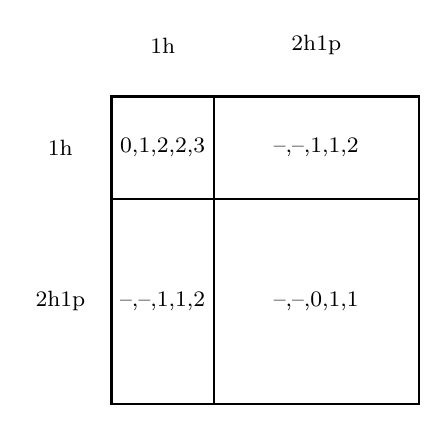
\begin{tikzpicture}[scale=1.3]
    \footnotesize
    %\draw [help lines] (-1,0) grid (23,5);
    \draw [thick] (0,0) rectangle (3,3);
    \draw [thick] (0,2) rectangle (1,3) node [midway] {0,1,2,2,3};
    \draw [thick] (1,0) rectangle (3,2) node [midway] {--,--,0,1,1};
    \draw [thick] (0,0) rectangle (1,2) node [midway] {--,--,1,1,2};
    \draw [thick] (1,2) rectangle (3,3) node [midway] {--,--,1,1,2};
    \node (1h1) at (0.5,3.5) {1h};
    \node (1h2) at (-0.5,2.5) {1h};
    \node (2h1) at (2.0,3.5) {2h1p};
    \node (2h2) at (-0.5,1.0) {2h1p};

\end{tikzpicture}

  \caption{}
  \label{}
\end{figure}
